% Chapter Template

\chapter{Implémentation et évaluation expérimentale} % Main chapter title

\label{ChapterX} % Change X to a consecutive number; for referencing this chapter elsewhere, use \ref{ChapterX}

%----------------------------------------------------------------------------------------
%	SECTION 1
%----------------------------------------------------------------------------------------

\section{Introduction}
Après avoir étudié le domaine de CBIR (les systèmes de recherche d’images
par le contenu ) et leur principe de fonctionnement, l’implémentation d’une application d’un système de recherche d’images devient une nécessité afin d’avoir une vue plus claire de ce que nous avons introduit dans les premiers chapitres. \\

Nous présenterons alors, dans ce chapitre, notre l’application,
les descripteurs utilisés et les bases d’images choisi afin de pouvoir évaluer notre système, ainsi les différentes étapes par lesquelles nous sommes passés pour sa réalisation.

\section{L’outil d’implémentation}
Dans la conception de notre application, nous avons choisi Python
comme langage de programmation, ce choix est justifié par plusieurs
facteurs, parmi eux on cite:
\begin{itemize}
	\item Une librairie très riche, il est complété par de multiples boîtes à outils (le calcul numérique matriciel avec Numpy, vision par ordinateur avec OpenCV, ...etc).
	\item Une syntaxe simple permettant une souplesse durant l'implémentation.
	\item Possible d’exécuter le code en dehors du programme (Testes unitaires).
	\item Une aide très bien faite.
	\item Opensource contrairement à Matlab.
\end{itemize}

\section{Les descripteurs d’image utilisés}
Pour la création de notre vecteur descripteur, nous avons utilisé des
caractéristiques de bas niveau comme déjà spécifier dans le chapitre 2. L'extraction se fait selon l'attribut visuel choisi: couleur, texture ou forme.
\subsection{Les descripteurs de couleur}
\textbf{Les modèles de couleur: }
Dans notre système, nous avons intégré l'espaces RGB(RVB) pour caractériser la couleur:\\

\begin{itemize}
	\item Le modèle RVB (Rouge, Vert, Bleu) : est l’espace de couleur le plus utilisé pour la représentation de la couleur. L’avantage d’utiliser ce modèle est que cette représentation est extrêmement basique, puisqu’aucun traitement n’est nécessaire.
\end{itemize}

Notre système présente à l'utilisateur les descripteurs suivants :
\begin{itemize}
	\item L'histogramme (RGB et HSV),
	\item Les moments statistiques.
\end{itemize}

\subsubsection{Histogramme}
Dans la création d’application, nous avons choisi d’utiliser les histogrammes par block dans l’espace RVB comme une technique de base.
On a quantifié chaque composant Rouge, Verte et Bleu de manière
équivalente à 17,17 et 17 block.

Le vecteur de caractéristiques est généralement de taille 17*17*17
\subsubsection{Les moments de couleur}
Pour enrichir les index de la couleur, nous avons utilisé les moments de
couleur au lieu de calculer la distribution complète. Dans cette étape, nous avons calculé les trois premiers moments de couleur (la moyenne et l’écart-type) pour chaque canal (R,G,B) dans le but de garder seulement les neuf valeurs obtenues, ainsi le vecteur de caractéristiques est de tailles 9.

\subsection{Les descripteurs de texture}
Pour caractériser la texture, nous avons choisi l'un des descripteurs classiques à savoir les mesures de Haralick basé sur les matrices de co-occurrence. De plus, nous avons intégré les filtres de Gabor comme étant l'un des descripteurs fortement utilisés dans la littérature.
\subsubsection{Les mesures de Haralick}
Les mesures de Haralick sont calculées à partir de la matrice de co-occurrence de l'image. Haralick décrit 14 statistiques qui peuvent être calculées à partir de la matrice de co-occurrence dans le but de décrire la texture de l'image [Site03]. Nous adoptant l'implémentation de la librairie Mahotas [Site04] qui met en œuvre seulement les 13 premières mesures. La dernière (14ème) est normalement considérée comme instable. Alors, le vecteur de caractéristiques est de taille 13.

\subsubsection{Les filtres de Gabor}
Dans le but d'améliorer les performances lié à la recherche basé sur la texture, nous avons utilisé les filtres de Gabor vue leurs robustesse prouvé par de nombreuse travaux de recherche dans la littérature.\\

Les filtres d'ondelettes de Gabor s'étendent sur 5 échelles (fréquences) : 0.06, 0.09, 0.13, 0.18, 0.25 avec huit orientations $ \theta_0 = 0, \theta_n = \theta_{n-1} + \frac{\pi}{8} , n = 1,...,7$  et qui sont appliqués sur l'image. La moyenne et l'écart-type des coefficients d'ondelettes de Gabor sont utilisés pour former un vecteur de caractéristiques de taille 5x8x2 = 240.

\subsection{Les descripteurs de forme}
Dans la partie basé sur la forme, nous avons intégré les moments de Hu comme descripteur classique et les moments de Zernike qui constitue une amélioration de performance comparant au moment de Hu.
\subsubsection{Moments de Hu}
Les moments de Hu sont basés sur les moments géométriques discutés dans le chapitre II section 2.2.3.\\
Si ƒ(x, y) est une image numérique, alors l'équation précédente devient:
\begin{equation}
\mu_{p,q} = \sum_{x=0}^{M-1}\sum_{y=0}^{N-1} (x- \bar{x})^p (y-\bar{x})^q f(x, y)
\end{equation}
D'où les moments géométriques (centraux):
\begin{figure}[H]
	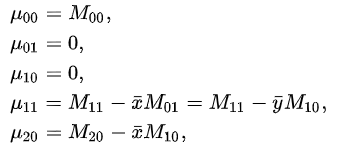
\includegraphics[width=0.5\textwidth]{momentCent} 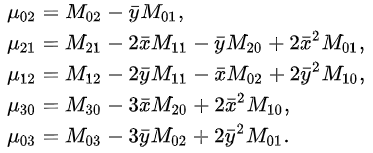
\includegraphics[width=0.5\textwidth]{momentCent1}
\end{figure}
Les moments $ \mu_{p,q} $ invariants en ce qui concerne à la fois la translation et l'échelle peuvent être construits à partir des moments géométriques en divisant par un moment central zéro-ième correctement mis à l'échelle :
\begin{equation}
\eta _{{ij}}={\frac  {\mu _{{ij}}}{\mu _{{00}}^{{\left(1+{\frac  {i+j}{2}}\right)}}}}\,\!
\end{equation}
où $ i + j \ge 2 $.
Comme le montre le travail de Hu, [Hu] les invariants en matière de translation, d'échelle et de rotation peuvent être construits :
\begin{figure}[H]
	\centering
	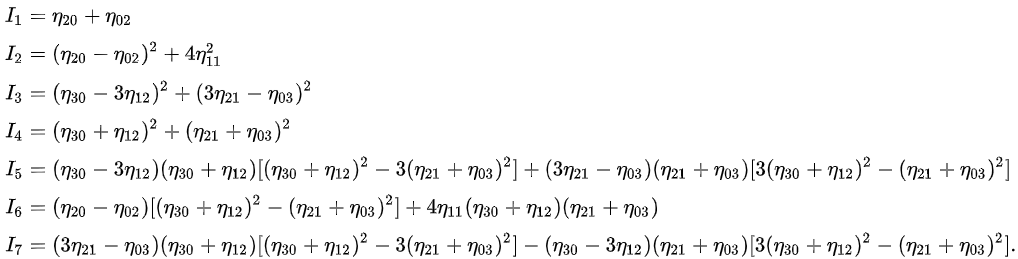
\includegraphics[width=1\textwidth]{huMom}
	\caption{Les moments de Hu.}
\end{figure}

Le vecteur de caractéristiques :
\subsubsection{Moments de Zernike}


Le vecteur de caractéristiques :
\section{Mesures de similarité}
Pour rechercher les images les plus similaires à une image requête, il faut pouvoir mesurer la similarité entre les images. Lorsqu’un utilisateur lance une recherche, le système effectue une mesure entre le vecteur descripteur de la requête et les vecteurs descripteurs des images de la base dans l’espace des attributs.\\

D'une façon générale, nous avons choisi d’utiliser les distances dérivées de la famille de distances de Minkowski; la distance de Manhatan et la distance Euclidienne.\\

Pour les distributions statistiques à savoir les histogrammes, nous avons ajouter la distances de $\chi^2$ (CHI-square)  .

\begin{table}[H]
	\centering
	\begin{tabular}{|c|c|c|}
		\hline
		\textbf{Distance} & \textbf{Formule}\\
		\hline
		\makecell{Manhatttan } & \makecell{\\
			$  d_1(I_1, I_2) = \sum_{i=1}^{N} \left|{I}_{1}(i)-{I}_{2}(i)\right|  $ }   \\
		\hline
		
		\makecell{Euclidienne} & \makecell{\\ $ d_2(I_1, I_2) =  \sqrt{\sum_{i=1}^{N} \left|{I}_{1}(i)-{I}_{2}(i)\right|^2} $}   \\
		\hline
		
		\makecell{$\chi^2$ (CHI-square)  } & 
			\makecell{\\
				$d(I_1, I_2)=\sum_{i=1}^{N} \frac{(I_1(i)-I_2(i))^2}{I_1(i)}$
			} \\   
		\hline
		
	\end{tabular}
	\caption{Les distances de Minkowski}
	
\end{table}
Ou :\\
$ I_1, I_2 $ sont les deux vecteurs de caractéristiques.\\
$ N $ est la dimension de vecteur.\\
$ i $ indice.

\section{Les bases d’mages utilisées }
\textbf{Corel-1000 - Wang:}
Cette base d’images contient 1000 images en couleurs. Ces images ont
été divisées en 10 classes de 100 images. Les thèmes représentés par les 10 classes sont : monuments, plage, autobus, dinosaures, aliments, éléphants, fleurs, chevaux, montagnes et l’Afrique.

\begin{figure}[h]
	\centering
	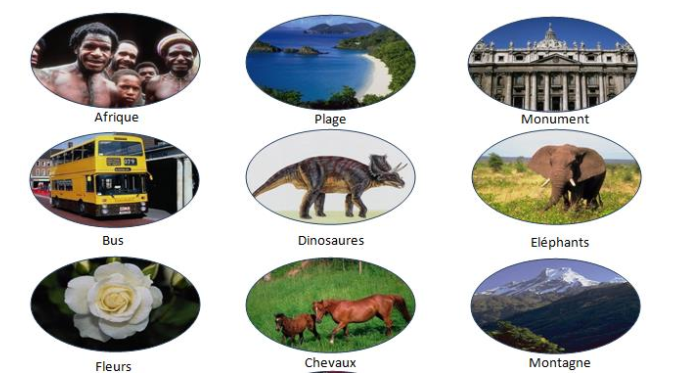
\includegraphics[width=0.6\textwidth]{wang} 
	\caption{Quelques images de la base d’image WANG.}
\end{figure}

\textbf{Columbia Object Image Library (COIL-100):}
Cette base d’images est très connue pour la reconnaissance des objets. Il y a deux bases d’images COIL : COIL-20 qui contient des images en niveaux de gris prises à partir de 20 objets différents et COIL-100 qui contient des images en couleurs prises à partir de 100 objets différents. Les deux bases d’images consistent en des images prises à partir des objets 3D avec des positions différentes. La base COIL-100 a 7200 images en couleurs (100 objets x72 images/objet). Chaque image a une taille de 128x128 pixels.

\begin{figure}[h]
	\centering
	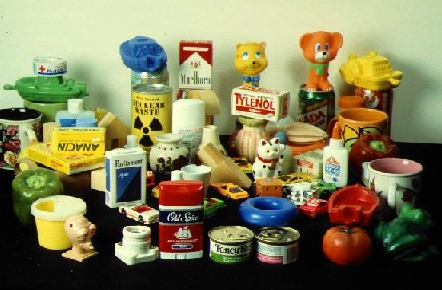
\includegraphics[width=0.6\textwidth]{coil} 
	\caption{Objets utilisés dans COIL-100.}
\end{figure}

\textbf{MIT1995 - VisTex:}
La base de données VisTex est une collection d'images de texture. La base de données a été créée dans le but de fournir un large ensemble de textures de haute qualité pour les applications de vision par ordinateur. En particulier, l'ensemble a été conçu comme une alternative à la bibliothèque de textures Brodatz, qui n'est pas disponible gratuitement pour la recherche [Site01]. L'objectif de VisTex est de fournir des images de texture qui sont représentatives des conditions du monde réel. Si VisTex peut remplacer les collections de textures traditionnelles, il comprend des exemples de nombreuses textures non traditionnelles. La base de données comporte plus de 100 images.

\begin{figure}[h]
	\centering
	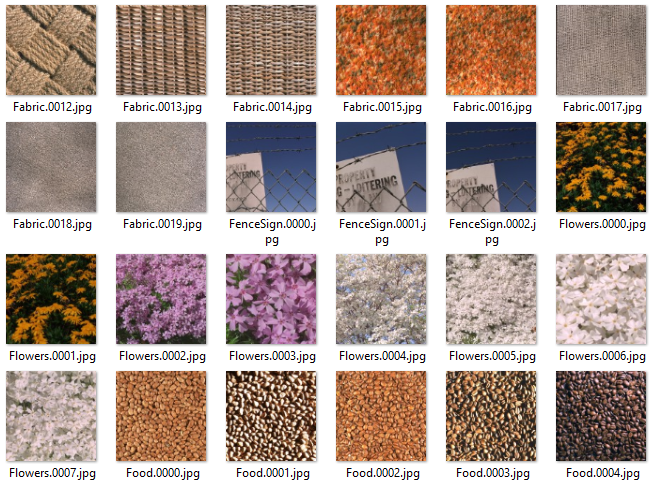
\includegraphics[width=0.6\textwidth]{VisTex} 
	\caption{Quelques images de la base d’image VisTex.}
\end{figure}

\textbf{MIT1995 - TRUNK12:}
Comme il n'existe pas d'ensemble de données d'images d'écorces d'arbres connu et accessible au public, un nouvel ensemble de données accessible au public a été créé dans le cadre de la thèse de Bsc [Site02]. Il contient environ 360 images d'écorces de 12 arbres différents qui se trouvent en Slovénie. Chaque classe d'arbres comprend environ 30 images au format JPEG, avec une résolution de 3000 x 4000 pixels. Toutes les images ont été prises avec l'appareil photo Nikon COOLPIX S3000 dans les mêmes conditions (distance de 20 cm, plusieurs arbres par classe, en évitant le bruit comme la mousse, mêmes conditions de lumière, prises en position verticale).

\begin{figure}[H]
	\centering
	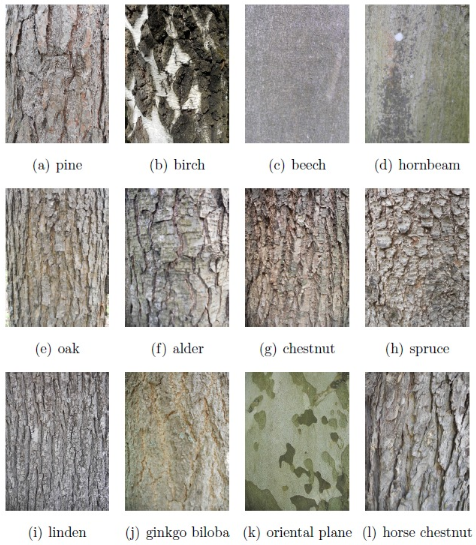
\includegraphics[width=0.6\textwidth]{trunk} 
	\caption{Quelques images de la base d’image TRUNK12.}
\end{figure}

\section{Mesure de la qualité des réponses}
Dans les systèmes de recherche d’images, une image est pertinente pour
une requête si les deux images sont dans la même classe.
La précision (ou valeur prédictive positive) est la proportion des items pertinents parmi l'ensemble des items proposés; le rappel (ou sensibilité) est la proportion des items pertinents proposés parmi l'ensemble des items pertinents. Ces deux notions correspondent ainsi à une conception et à une mesure de la pertinence.\\

Lorsqu'un moteur de recherche, par exemple, retourne 30 pages web dont seulement 20 sont pertinentes (les vrais positifs) et 10 ne le sont pas (les faux positifs), mais qu'il omet 40 autres pages pertinentes (les faux négatifs), sa précision est de 20/30 = 2/3 et son rappel vaut 20/(20+40) = 1/3.\\

La précision peut ainsi être comprise comme une mesure de l'exactitude ou de la qualité, tandis que le rappel est une mesure de l'exhaustivité ou de la quantité.\\


\begin{figure}[H]
	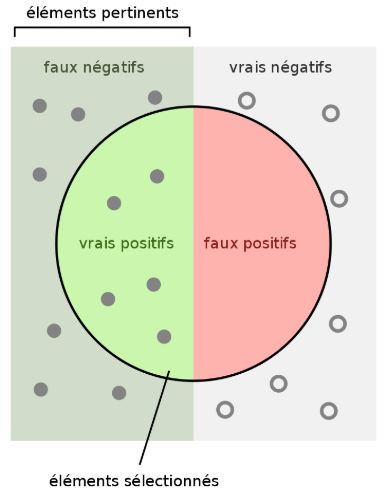
\includegraphics[width=0.5\textwidth]{recpre} 
	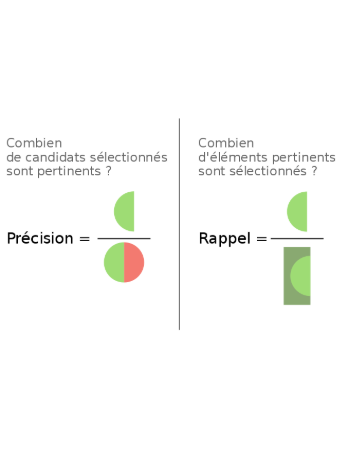
\includegraphics[width=0.5\textwidth]{recallprecision} 
	\caption{Rappel et précision.}
\end{figure}
Le rappel et la précision sont deux mesures très utilisées pour l’évaluation des performances d’un système CBIR. 

\begin{equation}
R = \frac{\text{VP}}{\text{FN et VP}} = \frac{\text{Nombre d'images pértinentes retrouvées} }{\text{Nombre total d'images pértinentes}}
\end{equation}
\begin{equation}
P = \frac{\text{VP}}{\text{VP et FP}} = \frac{\text{Nombre d'images pértinentes retrouvées}}{\text{Nombre total d'images retrouvées}}
\end{equation}
Ou: \\
VP: Vrais Positifs\\
VN: Vrais Négatifs\\
FP: Faux Positifs\\
FN: Faux Négatifs.
 
En statistique, la précision est appelée valeur prédictive positive et  le rappel est appelé sensibilité.

\section{Architecture de l’application}
Dans un système d’extraction d’images par le contenu il existe deux différents types de traitements :
\begin{itemize}
	\item \textbf{Traitement offline :}
	Ce type de traitement représente la phase de la construction de la base des signatures (d’attributs/vecteurs descripteurs).
	Cette opération est réalisée durant la construction du système.
	\item \textbf{Traitement online :}
	Ce type de traitement est effectué lors de l’introduction de la requête de l’utilisateur.
	Les signatures sont extraits de l’image requête puis comparés à ceux de la base de signatures qui a été déjà construite au préalable.
\end{itemize}
\begin{figure}[H]
	\centering
	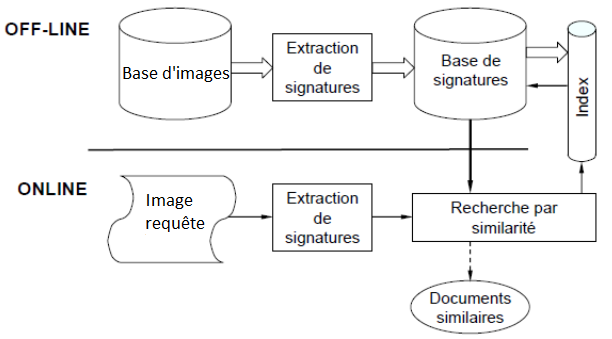
\includegraphics[width=0.8\textwidth]{architectureBDMM} 
	\caption{architecture de l’application.}
\end{figure}

\begin{figure}[H]
	\centering
	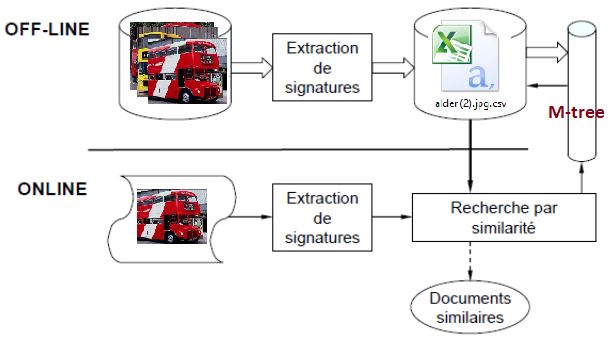
\includegraphics[width=0.8\textwidth]{architecture} 
	\caption{architecture de l’application avec utiles}
\end{figure}
\section{L’interface d’utilisateur }
Généralement, l'interface utilisateur de notre système permet à l'utilisateur des tâches comme:
 \begin{itemize}
 	\item Rechercher des images similaires à l'image requête (en ligne),
 	\item Indexer une bases d'images (hors ligne),
 	\item Calculer la qualité de chaque réponse ou requête,
 \end{itemize}

L'interface principale permet à l’utilisateur (Figure 4.8): 
\begin{itemize}
	\item Indexer une bases d'images (phase hors ligne) ou una bases de signatures,
	\item d’introduire son image requête,
	\item de choisir le descripteur à utiliser avec le type d'images en cas d'indexation d'une base d'images,
	\item de choisir la mesure de similarité à utiliser,
	\item de rechercher des images similaires à l'image requête (en ligne),
	\item de visualiser les images indexer pour en sélectionner la requête,
	\item de calculer la qualité de chaque réponse ou requête,
	\item de consulte la fenêtre aide pour savoir comment utiliser le système...etc.
\end{itemize}

\begin{figure}[H]
	\centering
	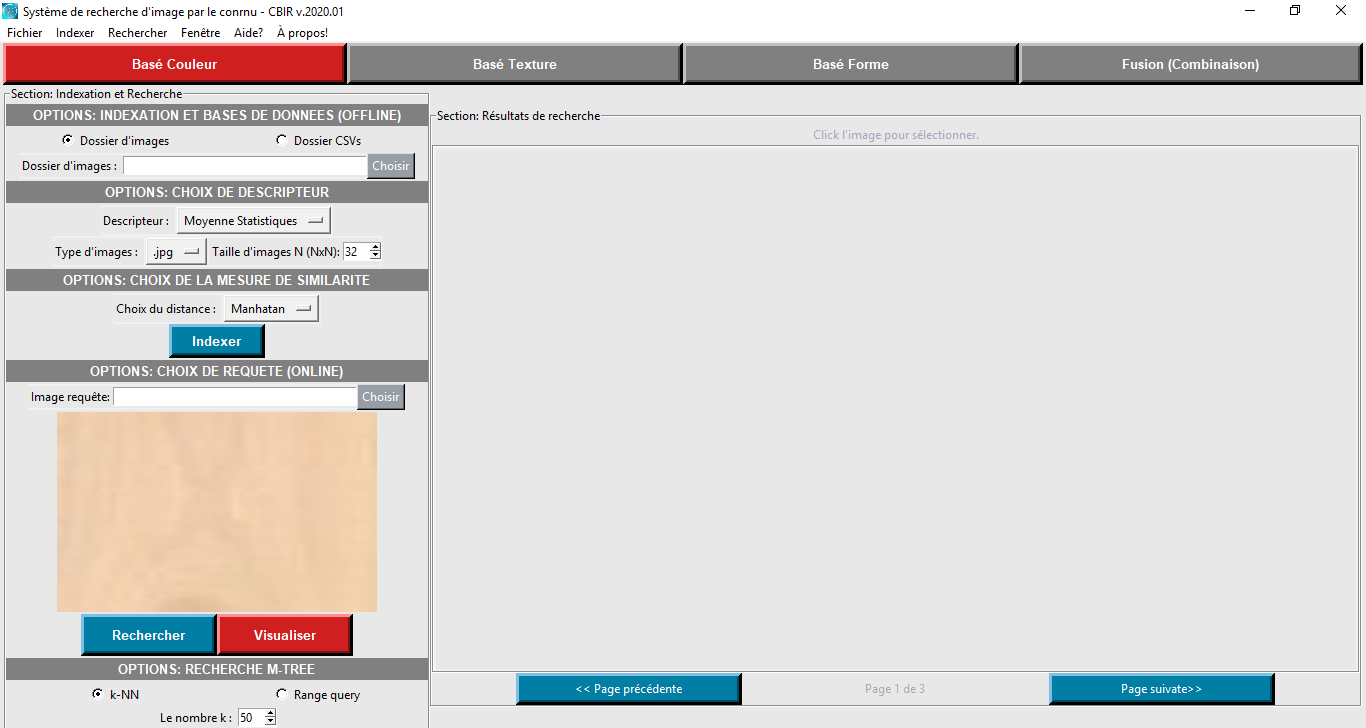
\includegraphics[width=1\textwidth]{gui} 
	\caption{L'interface d’utilisateur.}
\end{figure}
Après avoir choisi la base à indexer et les autres paramètres relatives à l'étapes d'indexations (descripteur, type d'images et mesure de similarité) l’utilisateur indexe cette base en appuyant sur la bouton 'Indexer'. Ainsi, l'indexation commence. \\\\

\begin{figure}[H]
	\centering
	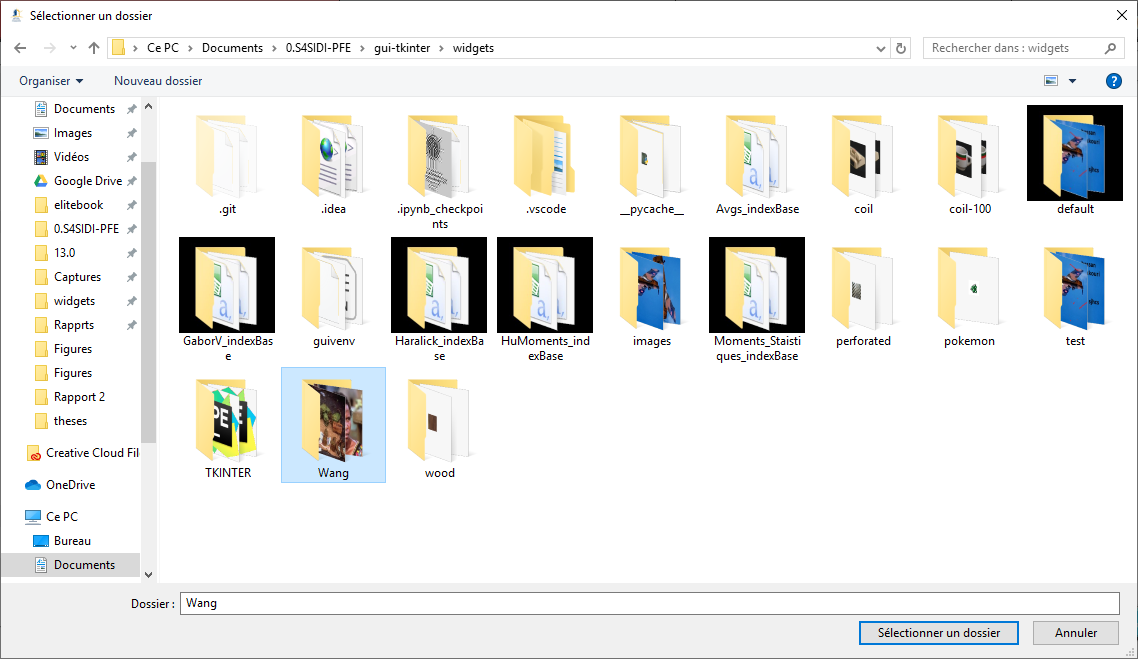
\includegraphics[width=1\textwidth]{browse folder} 
	\caption{Choix d'une base à indexer.}
\end{figure}

Une fois l'indexation est faite, l’utilisateur peut lancer une recherche après avoir choisi l'mage requête en appuyant sur la bouton 'Rechercher'. Pendant cette étape la signature de l’image est calculé pour l'utiliser dans l'un des requêtes de rechrche de la structure d'indexation M-Tree (Requête intervalle ou k-NN).\\

\begin{figure}[H]
	\centering
	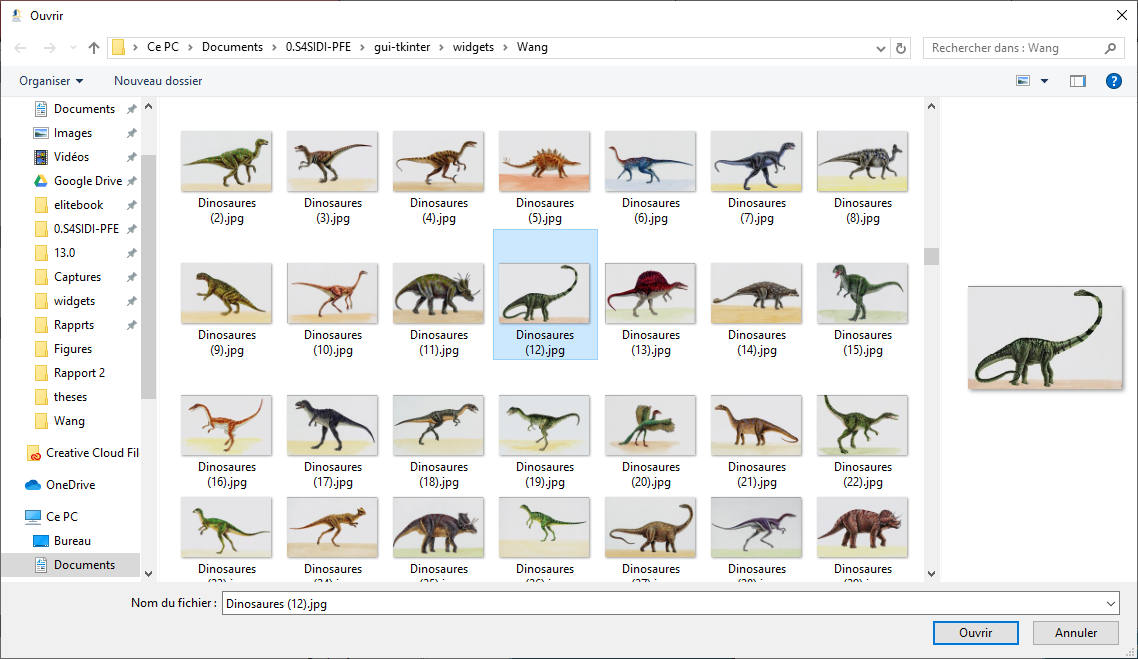
\includegraphics[width=1\textwidth]{browse query} 
	\caption{Choix de l'mage requête.}
\end{figure}
Résultas:
\begin{figure}[H]
	\centering
	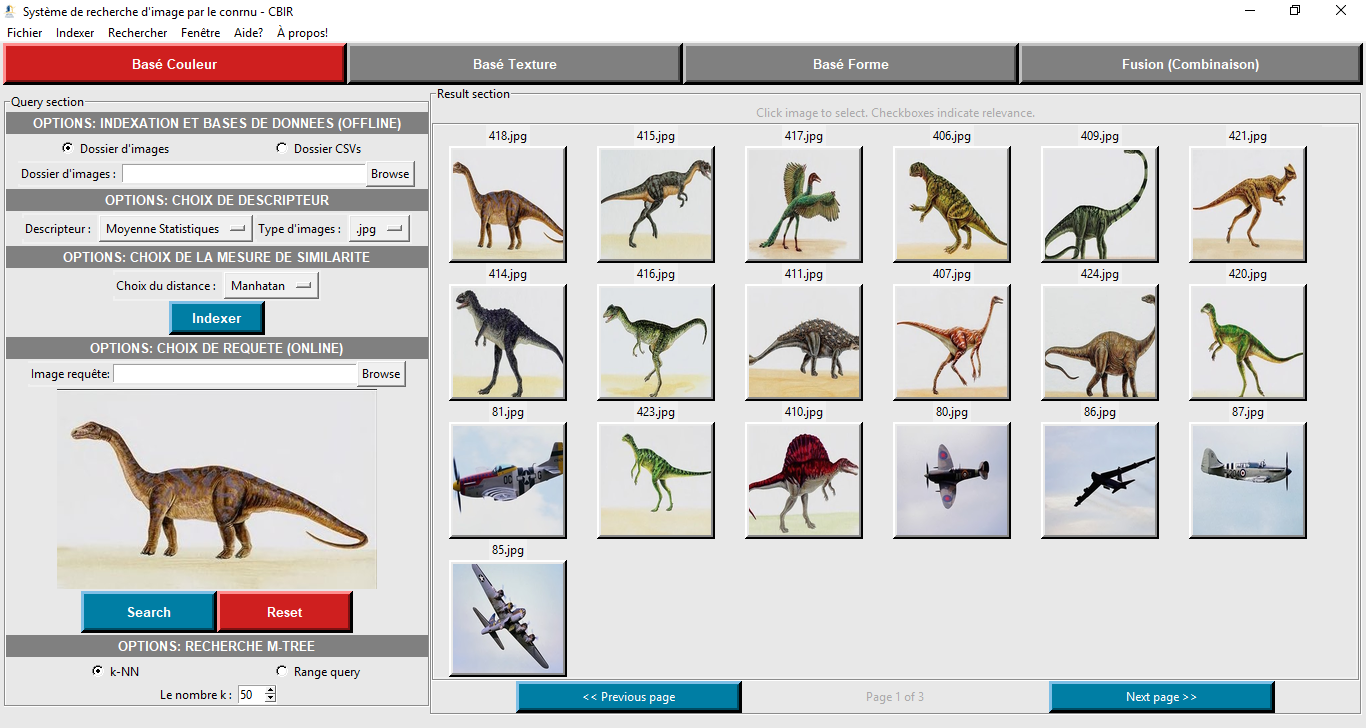
\includegraphics[width=1\textwidth]{query result} 
	\caption{L'interface d’utilisateur.}
\end{figure}

Le système affiche une liste d'images ordonnées par le degré de similarité.

Pour mesurer la qualité de la réponse on va vers le menu \textbf{fenêtre->mesures}:
\begin{figure}[H]
	\centering
	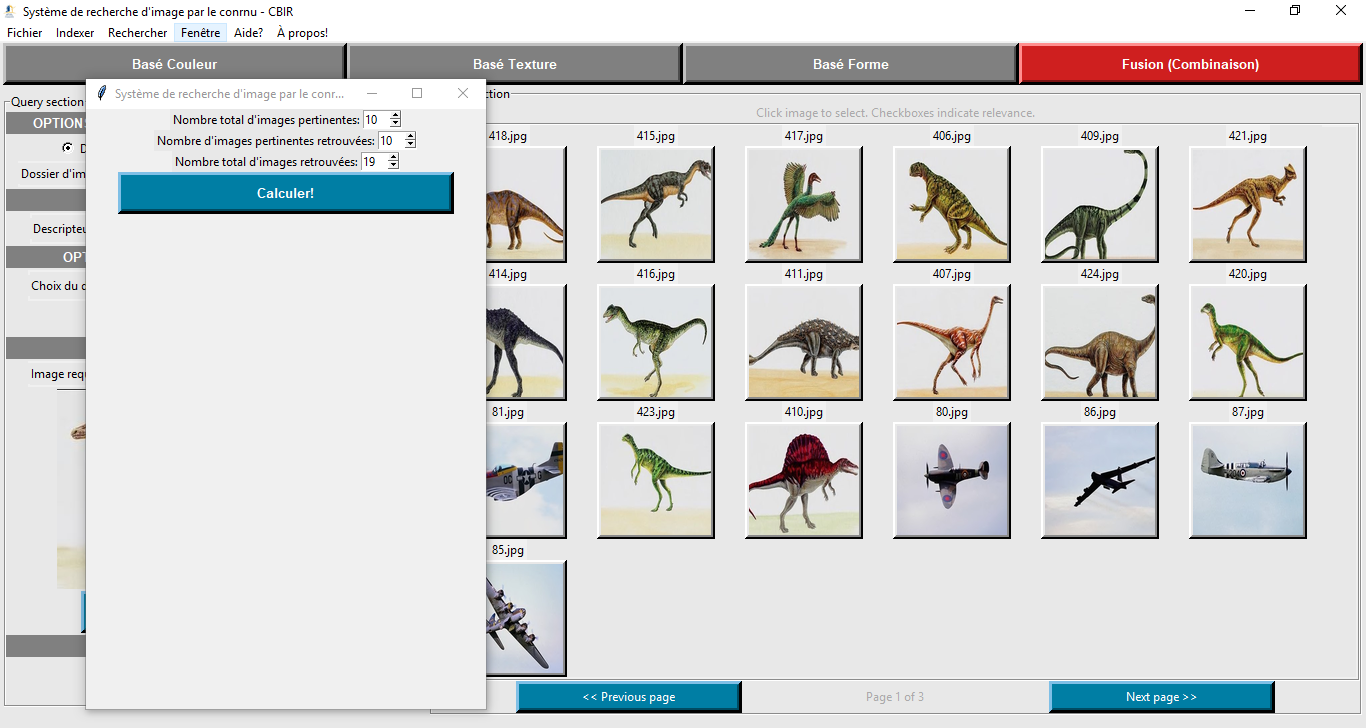
\includegraphics[width=1\textwidth]{mesuresQu} 
	\caption{L'interface d’utilisateur.}
\end{figure}
On calcule:
\begin{figure}[H]
	\centering
	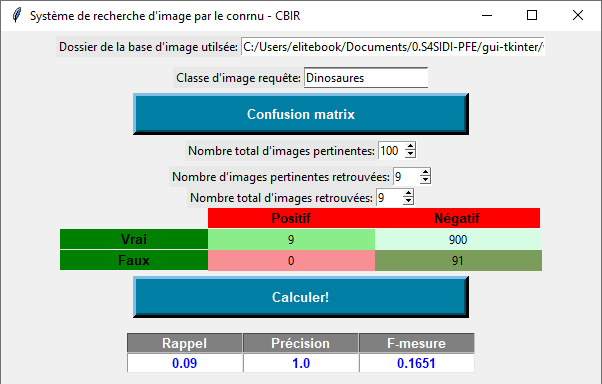
\includegraphics[width=1\textwidth]{QUresult} 
	\caption{L'interface d’utilisateur.}
\end{figure}

\section{Évaluation de système}
Nous avons testé la performance de chaque descripteurs utilisé et dans cette section nous avons présenté les différents résultats.

\paragraph{Processus suivi:}
Dans cette partie nous avons évalué l’application avec le calcule du rappel, la précision et F-mesure pour chaque image requête. Le principe de fonctionnement est simple; les images requêtes son sélectionnées de manière aléatoires (sans répétition de la même image requête) et on calcul les mesures de pertinence. Nous choisissons la base de donnée coil-100 pour comparer entre les descripteurs. 
\subsection{Descripteurs de la couleur}
Nous avons effectué un ensemble de tests sur 50 images requêtes (5 images
pour chaque classe) ou chaque image est sélectionnée de manière aléatoire
sans répétition. La précision de chaque classe est calculée par la moyenne
des précisions de ses images. Puis à la phase finale, on peut déduire la
précision globale de système qui représente la moyenne de toutes les classes.



\subsection{Descripteurs de la texture}
\subsection{Descripteurs de la forme}
\subsection{Descripteurs combinés}
\section{Problèmes rencontré}
\section{Perspective}
\section{Conclusion}
Au cours de ce dernier chapitre, nous avons réalisé un programme de
recherche d’images par le contenu en essayant d’utiliser les descripteurs les plus recommandés. Le test a été effectué avec une base d’images
universellement connu. La comparaison de nos résultats avec ceux de la
littérature permet de valider notre travail.